\subsection{Gestion de la bibliographie}
Pour la gestion de la bibliographie au sein du document,
nous utilisons le package \texttt{biblatex}.
Celui-ci permet d'écrire l'ensemble de nos références dans un fichier \texttt{.bib}
sous la forme suivante.
\begin{verbatim}
  @online{histoire_mod_plantes,
    title = {Une histoire de la modélisation des plantes},
    author = {Philippe de Reffye and Marc Jaeger 
    and Paul-Henry Cournède},
    url = {https://interstices.info/jcms/c_38032/une-histoire-de-
    la-modelisation-des-plantes},
    year = {2009},
    month = "04",
  }
\end{verbatim}
La mise en page est alors automatique en fonction des informations fournies
et le rendu de l'exemple est présenté ci dessous.
\begin{figure}[h]
  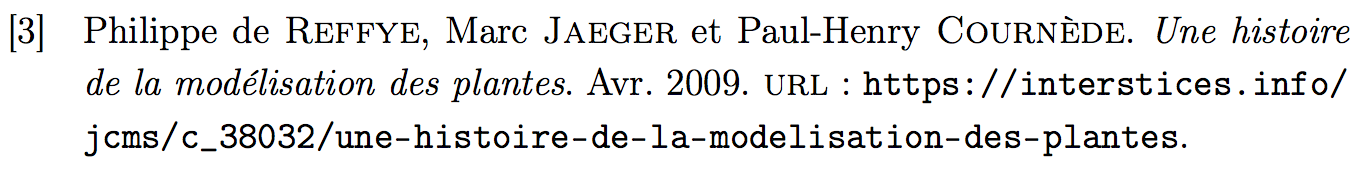
\includegraphics[scale=0.6]{./img/rendu_elem_bib.jpg}
\end{figure}

Cela parait à priori assez lourd d'écrire soi-même toutes les informations
en suivant cette syntaxe mais il existe des logiciels comme Zotero
qui font le travail à notre place.
Les sources trouvées sur Google Scholar peuvent également être exportées
aisément au format \texttt{BibTex}.
